% Die Beamer-Klasse unterstützt folgende Optionen, die von
% besonderem Interesse sind (alle Standardoptionen werden
% ebenfalls unterstützt; siehe beamer-Basisdokumentation):
% 
%%%%%%%%%%%%%%%%%%%%%%%%%%%%%%%%%%%%%%%%%%%%%%%%%%%%%%%%%%%%%%%
% aspectratio: Seitenverhältnis des resultierenden Dokuments
% (Achtung: Aufgrund der Designvorgaben ergeben sich unterschiedliche
% Größen der effektiv nutzbaren Textblöcke)
%
% Standardeinstellung: 'aspectratio=43'
%
% Mögliche Einstellungen:
% 'aspectratio=43'   (4:3)
% 'aspectratio=169'  (16:9)
% 'aspectratio=1610' (16:10)
% 
%%%%%%%%%%%%%%%%%%%%%%%%%%%%%%%%%%%%%%%%%%%%%%%%%%%%%%%%%%%%%%%
% fontsize: Basisschriftgröße (Größen für Überschriften etc. werden
% aus dieser Basis automatisch abgeleitet)
%
% Standardeinstellung: '22pt' (entspricht den Design-Vorgaben; sehr groß!)
%
% Mögliche Einstellungen:
% '8pt', '9pt', '10pt', '11pt', '12pt', '14pt', '16pt',
% '17pt','20pt','22pt', '24pt', '26pt', '28pt'

\documentclass[aspectratio=169,16pt,xcolor=table]{beamer}

% Der OTHR-Theme unterstützt folgende Optionen:
% 
%%%%%%%%%%%%%%%%%%%%%%%%%%%%%%%%%%%%%%%%%%%%%%%%%%%%%%%%%%%%%%%
% department: (Wahl der Abteilung/Fakultät)
%
% default: 'OTHR'
%
% Mögliche Einstellungen:
% 'FakA', 'FakAM', 'FakB', 'FakBW', 'FakEI', 
% 'FakIM', 'FakM', 'FakS', 'ZWW', 'IPF',
% 'SappZ', 'KNB', 'ReMIC', 'LFD', 'LAS3',
% 'DK0PT', 'LBM', 'LeanLab', 'LFT', 'LFW',
% 'LMP', 'LMS', 'LRT', 'LWS', 'RRRU',
% 'RST', 'CEEC', 'FEM', 'IST'
%%%%%%%%%%%%%%%%%%%%%%%%%%%%%%%%%%%%%%%%%%%%%%%%%%%%%%%%%%%%%%%%%
% headerMode: Aussehen und Inhalt der Kopfleiste
%
% Standardeinstellung: 'full'
%
% Mögliche Einstellungen:
% 'full', 'frametitle', 'frametitleSection'
% 

%%%%%%%%%%%%%%%%%%%%%%%%%%%%%%%%%%%%%%%%%%%%%%%%%%%%%%%%%%%%%%%%%
% Binäre Schalter (können angegeben oder nicht angegeben werden;
% Standardeinstellung: Nicht angegeben)
%
%%%%%%%%%%%%%%%
% navbar: Navigationssymbole anzeigen (Seite vor/zurück, Kapitel vor/zurück etc.)

% pageNumbers: Seitennummerierung

% blackFont: Nur schwarze Schriftfarbe verwenden (ansonsten: Fakultätsfarben)

% frametitleCenter: Titel in der Kopfzeile zentrieren (ansonsten: rechtsbündig)
\usepackage{csquotes}

\usetheme[department=FakIM,pageNumbers]{OTHR}

% Inhaltsspezifische Zusatzpakete laden 
\usepackage[ngerman]{babel}
\usepackage[utf8]{luainputenc}
\usepackage{lipsum}
\usepackage{graphicx}
\graphicspath{ {./img/} }
\usepackage{amsmath}
\usepackage{adjustbox}
\usepackage{xcolor}
\usepackage{ulem}
\usepackage[usestackEOL]{stackengine}
\usepackage{hyperref}
\usepackage[backend=bibtex,style=numeric]{biblatex}
\usepackage{breakcites}
\usepackage{etoolbox}
\usepackage{multimedia}
\usepackage{media9}
%\usepackage{csquotes}
% tables
%\catcode30=12
\usepackage{tabularx}

\renewcommand\bibfont{\tiny}
\addbibresource{ref.bib}
%\bibliographystyle{IEEEtran}

\patchcmd{\thebibliography}{\footnotesize}{\tiny}{}{}

\newcommand{\tabitem}{~~\llap{\textbullet}~~}
% this adds the content table for each section
\AtBeginSection[]
{
  \begin{frame}[allowframebreaks]
    \frametitle{Inhalt}
    \tableofcontents[currentsection]
  \end{frame}
}

\date{15. Januar 2024}

\begin{document}

\begin{frame}
  \begin{figure}[h!]
    \centering   
	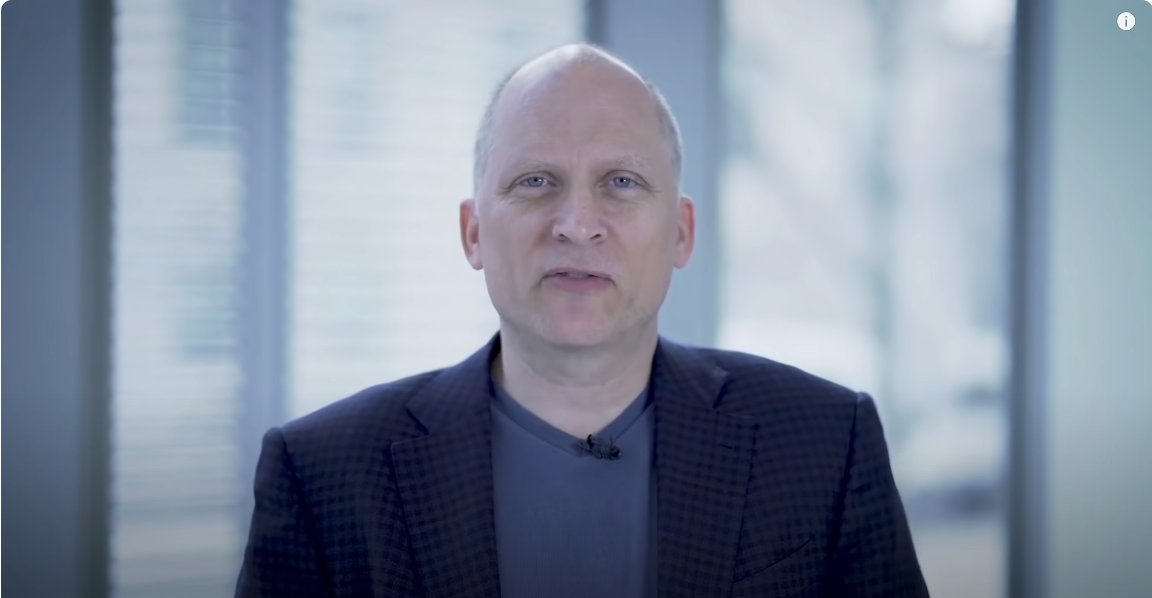
\includegraphics[width=0.8\textwidth]{pictures/Video_Vorschau.png}
  \end{figure}
\end{frame}

\begin{frame}
  \begin{figure}[h!]
    \centering   
	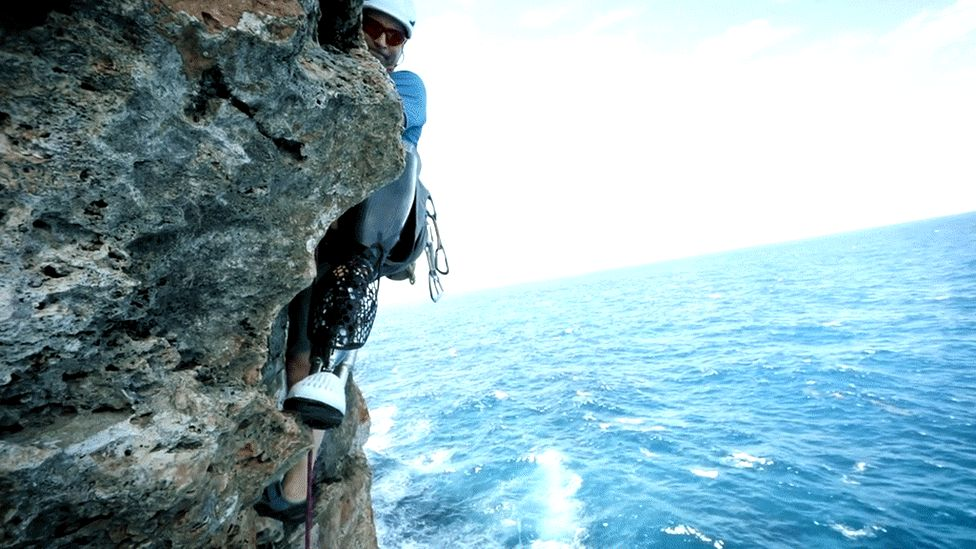
\includegraphics[width=0.8\textwidth]{pictures/AMI_Klettern.png}
  \end{figure}
\end{frame}

\title{Transhumanismus}
\subtitle{Fortschritt oder Dystopie?}
\author{Marcel Ott, Nicolas Zander, Lorenz Branner, Severin Bittl, Thomas Gailinger}
\institute{Ethik in der Informatik}

\maketitle

\begin{frame}[allowframebreaks]
	\frametitle{Inhaltsverzeichnis}
	\tableofcontents
\end{frame}

\section{Einleitung}
\subsection{Begriffserläuterungen}
\begin{frame}
	\frametitle{Begriffserläuterungen}
	\begin{itemize}
	  \item Transhumanismus
    \begin{itemize}
      \item Ausschöpfung der natürlichen menschlichen Grenzen mit Wissenschaft~\cite{Merzlyakov2022}\\
      => Beibehaltung der Grundform des Menschen
    \end{itemize}
	\item Posthumanimus
    \begin{itemize}
      \item Überwindung der menschlichen Grenzen~\cite{Merzlyakov2022}\\
      \item Mensch ist eine Sackgasse und Cyborg wird als nächster Schritt der Evolution angesehen~\cite{Merzlyakov2022}\\
      => Grundform des Menschen wird abgeschafft
    \end{itemize}
    \item Cyborg
    \begin{itemize}
      \item Integriertes System aus menschlichen und maschinellen Teilen~\cite{warwick2000cyborg}
    \end{itemize}
	\end{itemize}
  \scriptsize Grenzen zwischen Transhumanismus und Posthumanismus sind jedoch fließend werden, aber oft synonym verwendet, was jedoch aufgrund der Unterschiede von vielen Forschern kritisiert wird~\cite{Merzlyakov2022}
\end{frame}

\subsection{Was ist normal?}
\begin{frame}
  \frametitle{Was ist normal?}
  Prof. Dr. Anette Breczko: Die Überwachung biotechnologischer Möglichkeiten erfordert zweifellos eine Unterscheidung zwischen "therapeutischen'' und "Verbesserungs''-Aktivitäten~\cite{breczko2021human}
  
  \vspace{12pt}
  \textbf{Zentrale Frage hierfür:} Was ist normal? 
\end{frame}

\begin{frame}
	\frametitle{Was ist normal?}
  \textbf{Was ist normal?}

  \vspace{12pt}
  \small Erscheint intuitiv als triviale Frage mit folgenden Antworten:
	\begin{itemize}
	  \item Statischer Durchschnitt
	  \item Mehrheit
	  \item Herrschende Klasse z. B. POC als minderwertig bei Sklaverei
  \end{itemize}
\end{frame}

\begin{frame}
	\frametitle{Was ist normal?}
  \small Genannte Punkte machen jedoch wenig Sinn: 
	\begin{itemize}
	  \item Schildmann (Erziehungswissenschafterlin): Normalität ist sehr indiviuell und vom Selbst oder der umgebenden Gruppe bestimmt s. Cochlea-Implantat~\cite{schildmann1999normal}
	  \item Aguayo-Krauthausen (Aktivist): Behinderung als Eigenschaft, wie die Augenfarbe wahrnehmen~\cite{aguayo2023inklusion}
	  \item Ethische Grundaussagen der Lebenshilfe: ``Es ist normal, verschieden zu sein.''~\cite{lebenshilfeFlyer}
  \end{itemize}
\end{frame}

\subsection{Einige Chancen des Transhumanismus}
\begin{frame}
	\frametitle{Einige Chancen des Transhumanismus}
  \textbf{Einige Chancen des Transhumanismus:}
	\begin{itemize}
    \item Heilen von Krankheiten z. B. mittels DBS~\cite{perlmutter2006deep}, TBS~\cite{hallett2007transcranial} und Nanobots~\cite{wang2022intelligent}
    \item Steigerung der physischen und kognitiven Leistungsfähigkeit z. B. Prüfungsleistungen mittels TMS verbessern~\cite{luber2014enhancement} oder erhöhte Ausdauer ~\cite{kurzweil2005singularity}
    \item Anpassungen auf Vorstellungen des Individuums z. B. Charaktereigenschaften auf eigenen Wunsch ändern~\cite{logtenberg2022beyond}\\    
  \end{itemize}
  \small \textbf{Kapitalitisher Grundgedanke:} stetige Verbesserung ist eine zentrale Voraussetzung für Wachstum und wieso bei Produkten aufhören?
\end{frame}

\section{Ethische Fragestellungen des Transhumanismus}
\subsection{Selbstbestimmung des Individuums}
\begin{frame}
  \frametitle{Selbstbestimmung des Individuums}
  \textbf{Selbstbestimmung des Individuums:}
  \begin{itemize}
    \item \textbf{Recht auf freie Entfaltung:} Jeder hat das Recht auf freie Entfaltung, solange die Rechte anderer oder bestehendes Recht nicht verletzt werden~\cite{fur1996grundgesetz}.
    \begin{itemize}
      \item \textit{Individuelle Identität:} Menschen können ihre eigene Identität frei wählen.
      \item \textit{Natürlichkeit bewahren:} Der Wunsch, in seiner natürlichen Form zu bleiben, ist ein essentieller Aspekt.
    \end{itemize}
    \item \textbf{Freie Entscheidung in einer Welt der Verbesserung:} In einer Gesellschaft, in der die Mehrheit von Enhancements profitiert, könnten jene, die sich dagegen entscheiden, im Alltagsleben benachteiligt sein z. B. Profi Bodybuilding und der Einsatz von Steroiden
  \end{itemize}
\end{frame}

\subsection{Entscheidungen treffen für andere}
\begin{frame}
  \frametitle{Entscheidungen treffen für andere}
  \textbf{Entscheidungen treffen für andere:}
  \begin{itemize}
    \item Schwierigkeit der Entscheidungsfindung vor Allem bei Verbesserungen~\cite{plavsienkova2021healthy}
    \item Individuelle Abwägung von Nebenwirkungen
    \item Gesellschaftliche Verantwortung z.B. höhere Gesundheitskosten für alle\\
    => Mögliche Pflicht zur Verbesserung
    \item Herausforderung bei Personen die nicht selbstbestimmt entscheiden können z. B. Locked-in-Syndrom~\cite{das2022locked} oder Kinder
    \textbf{Entscheidungen gegen Verbesserungen könnten zu massiven Nachteilen im späteren Leben führen}
  \end{itemize}
\end{frame}

\subsection{Fallbeispiel: Entscheidungen für ein Kind}
\begin{frame}
  \frametitle{Fallbeispiel: Entscheidungen für ein Kind}
  \textbf{Fallbeispiel: Entscheidungen für andere treffen}
  \begin{itemize}
    \item Gerichtsverhandlung wegen Entscheidung gegen ein Cochlea-Implantat bei gehörlosen Eltern~\cite{brde}
    \item Die Klinik sah die Ablehnung als Gefährdung des Kindeswohls und leitete ein Kinderschutzverfahren ein.
    \item Familiengerichtsentscheidung am 29. Januar 2019:
    \begin{itemize}
      \item Keine familienrechtlichen Maßnahmen aufgrund unzureichender Gründe.
      \item Eltern können den optimalen Therapieverlauf nach der Implantation nicht gewährleisten.
      \item Ohne Akzeptanz der Eltern ist es unmöglich, dass das Kind trotz Cochlea-Implantat die Hör- und Sprachfähigkeit erlangt.~\cite{brde}
    \end{itemize}
  \end{itemize}
\end{frame}

\subsection{Autonomie einer Gruppe}
\begin{frame}
  \frametitle{Autonomie einer Gruppe}
  \textbf{Autonomie einer Gruppe:}
  \begin{itemize}
    \item Anliegen derjenigen, die sich gegen Normalisierung entscheiden, finden kaum Beachtung mehr. (Argument der leichteren Lösung)
    \item Minderheiten und Gruppen haben ihre eigene kulturelle Dynamik, die durch Normalisierung verloren gehen\\z. B. Gehörlosen-Community, die eine einzigartige Kommunikationsform pflegt und geschätzt werden sollte~\cite{lee2016cochlear}.
    \item Technologie ermöglicht betroffenen Gruppen selbstbestimmtes leben~\cite{das2022locked}.
  \end{itemize}
\end{frame}

\subsection{Unabschätzbare Folgen}
\begin{frame}
  \frametitle{Unabschätzbare Folgen}
  \textbf{Unabschätzbare Folgen:}\\
  \small Neue Technologien bringen oft unvorhergesehene Folgen mit sich z.B. FCKWs wurden als Kälte- und Treibmittel genutzt und führten zur Entstehung des Ozonlochs~\cite{rowland1996stratospheric}
  Beispiele beim Transhumanismus:
  \begin{itemize}
    \item DNA-Veränderungen
    \begin{itemize}
      \item Unvorhersehbare Folgen bei DNA-Veränderungen\\
      => fatale und irreversible Auswirkungen auf den Körper
    \end{itemize}
    \item DBS
    \begin{itemize}
      \item Komplexität und mangelndes Wissen des Gehirns führt zu unerwünschten Nebenwirkungen, wie Depressionen oder Suizid~\cite{zarzycki2020stimulation}.
      \item Elektroden stimulieren großflächig, was zu ungewollten Stimulationen benachbarter Gehirnareale führen kann.
    \end{itemize}
  \end{itemize}
\end{frame}

\subsection{Gesundheit und darüber hinaus}
\begin{frame}
  \frametitle{Gesundheit und darüber hinaus}
  \textbf{Gesundheit und darüber hinaus:}\\
  Allgemein gilt:
  \begin{itemize}
      \item Sehr eingeschränktes Wissen über Funktionsweise vom menschlichen Körper
      \item Eingriffe bergen ein gewisses Risiko, z.B. Misserfolg, Verletzungen, Tod
      \item Irreversibilität ist besonders bedenklich, z.B. bei BMI, DBS
  \end{itemize}
  Wiederherstellen des ``Normalzustandes'':
  Kranke Menschen haben starke Einschränkungen im Alltag und bei der Gestaltung ihres Lebens, daher wird Risiko des Eingriffs oftmals in Kauf genommen
\end{frame}

\begin{frame}
  \frametitle{Gesundheit und darüber hinaus}
  \begin{textblock*}{15cm}(1cm,1.3cm)
    Erweiterung der Fähigkeiten:
    \begin{itemize}
        \item Dem Eingriffsrisiko steht nun der Vorteil der Verbesserung gegenüber
        \item Irreversibilität vermeidet möglicherweise künftige Eingriffe
    \end{itemize}
  \end{textblock*}
  \begin{picture}(0,0)
    \put(100,-180){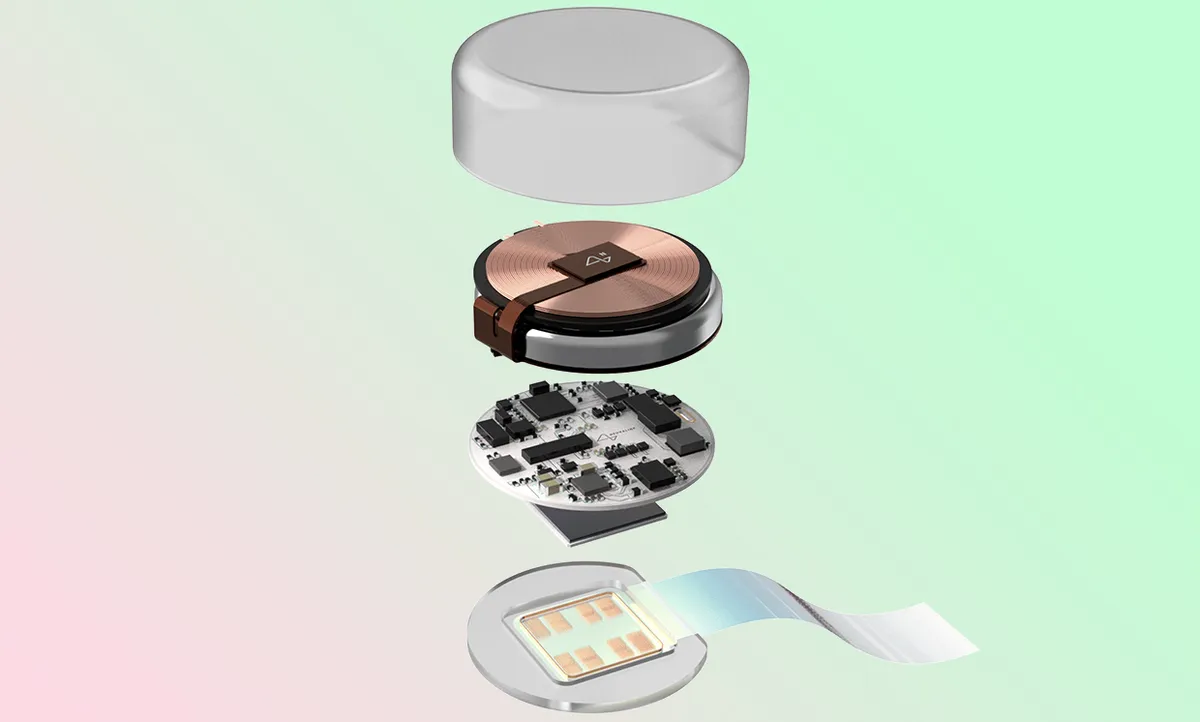
\includegraphics[scale=0.15]{./pictures/neuralink.png}}
  \end{picture}
  \vspace{6.2cm}
  \begin{flushleft}
      \tiny Quelle: \url{https://spectrum.ieee.org/elon-musk-brain-neuralink}, zuletzt besucht am 21.12.2023
  \end{flushleft}
\end{frame}

\subsection{Gesellschaftliche Spaltung unausweichlich?}
\begin{frame}
  \frametitle{Gesellschaftliche Spaltung unausweichlich?}
  \small \textbf{Gesellschaftlichespaltung unausweichlich?}\\
  \small Probleme bei der Finanzierung und Vertrieb von transhumanistischer Technik~\cite{khan_aziz_2019}:
  \begin{itemize}
    \item Gesellschaft finanziert Verbesserungen? Kranke werden benachteiligt
    \item Private Organisationen? Unkontrollierte Ausbreitung möglich
    \item Der Einzelne? Viele haben nicht die finanziellen Mittel
  \end{itemize}
 \end{frame}

\begin{frame}
  \frametitle{Gesellschaftlichespaltung unausweichlich?}
  \small \textbf{Gesellschaftlichespaltung unausweichlich?}\\
  \small Aktuelle Situation: Gesell. Spaltung zwischen Arm und Reich\\
  \small \textbf{Vergleich Lebenserwartung bei Männern}~\cite{lampert2014}:
  \begin{itemize}
    \item Reiche: 80,9 Jahre
    \item Arme: 70,1 Jahre
  \end{itemize}
  \small Gründe für die Unterschiede:
  \begin{itemize}
    \item Bessere ärztliche Versorgung für Reiche
    \item Keine finanziellen Probleme bei teuren Medikamenten
    \item Zugang zu gesunder (teurer) Ernährung
  \end{itemize}
\end{frame}

\subsection{Zukunft der Gesundheitsversorgung}
\begin{frame}
  \frametitle{Zukunft der Gesundheitsversorgung}
  \small \textbf{Zukunft der Gesundheitsversorgung}\\
  Prognose: Die Spaltung in der Gesellschaft nimmt zu.
  Neue Organe, Tissue-Engineering, Verjüngungsmedikamente, Mikroroboter sind nur für einen (wohlhabenden) Teil der Bevölkerung verfügbar.
  \textbf{Negative Folgen transhumanistischer Technologie~\cite{khan_aziz_2019}:}
  \begin{itemize}
      \item Nachteile überwiegen die Vorteile
      \item Gefahr der Verschiebung der Gesundheitsversorgung in private Hände
  \end{itemize}
\end{frame}

\subsection{Ethische Forschung und wie es aktuell läuft}
\begin{frame}
  \frametitle{Ethische Forschung und wie es aktuell läuft}
  \textbf{Ethische Forschung und wie es aktuell läuft:}
  Entwicklung transhumanistischer Technologie
  \begin{itemize}
    \item Die Entwicklung transhumanistischer Technologie ist vergleichbar mit der Entwicklung von Impfstoffen oder Medikamenten – teuer und langwierig.
    \item Die Zulassung solcher Technologien erfolgt nur mit Tests an Menschen.
    \item Starke Regulierungen in vielen Ländern, um die möglichen Testteilnehmer zu schützen.\\
    => Mögliche Verlagerung der Entwicklung in wirtschaftlich schwächere Länder und damit verbundene Ausbeutung der dortigen Bevölkerung.
  \end{itemize}
\end{frame}

\begin{frame}
  \begin{itemize}
      \item Es besteht eine extreme Neigung zu transhumanistischer Technologie.
      \item Risiken könnten vernachlässigt werden.
  \end{itemize}
\end{frame}

\section{Risikoberwertung}
\subsection{Regulierungen}
\begin{frame}{Regulierungen}
    \textbf{Regulierungen}
    \begin{itemize}
      \item{Regulierungen, rechtliche Rahmenbedingungen und Ethikcodizes nötig}
      \item{AI Act der EU 2021~\cite{ai_act_eu_2021} und Fortschritte damit~\cite{ai_act_deal_2023}}
      \item{Seit einigen Jahren im Diskurs anhand vergleichbarer Fälle~\cite{lee2016cochlear}}
    \end{itemize}
\end{frame}

\subsection{Risiken}
\begin{frame}{Risiken}
Risiken
    \begin{table}
    \centering
         \setlength{\leftmargini}{0.4cm}
       \begin{tabular}{| m{4cm} | m{4cm} | m{4cm}|}
        \hline
        \footnotesize{Individuum} & \footnotesize{Organisationen} & \footnotesize{Gesellschaft} \\ 
        \hline
        \begin{itemize}
        \item \scriptsize{Folgen von Hackerangriffen~\cite{khan_aziz_2019}} 
        \item \scriptsize{ Eigengefährdung von Nutzenden~\cite{khan_aziz_2019}}
        \item \scriptsize{ Unbekannte Langezeitfolgen~\cite{Burwell:2017aa}}
        \end{itemize}
        & 
        \begin{itemize}
        \item \scriptsize{Kapitalgetriebene Entscheidungen~\cite{khan_aziz_2019}} 
        \item \scriptsize{ Neuro-Marketing~\cite{khan_aziz_2019}}
        \item \scriptsize{ Monopolbildung~\cite{khan_aziz_2019}}
        \end{itemize}
        &
        \begin{itemize}
        \item \scriptsize{Unfairen Vorteil verschaffen~\cite{khan_aziz_2019} }
        \item \scriptsize{ Militante Interessen~\cite{khan_aziz_2019}}
        \item \scriptsize{ Verlust Autonomie und Menschlichkeit~\cite{Burwell:2017aa}}
        \end{itemize}
        \\
        \hline
    \end{tabular}
    \end{table}
\end{frame}
%%%THOMAS

\section{EU-Riskoklassen}
\subsection{AI-Act}
\begin{frame}{AI-Act}
    \begin{center}
               \raisebox{8cm}{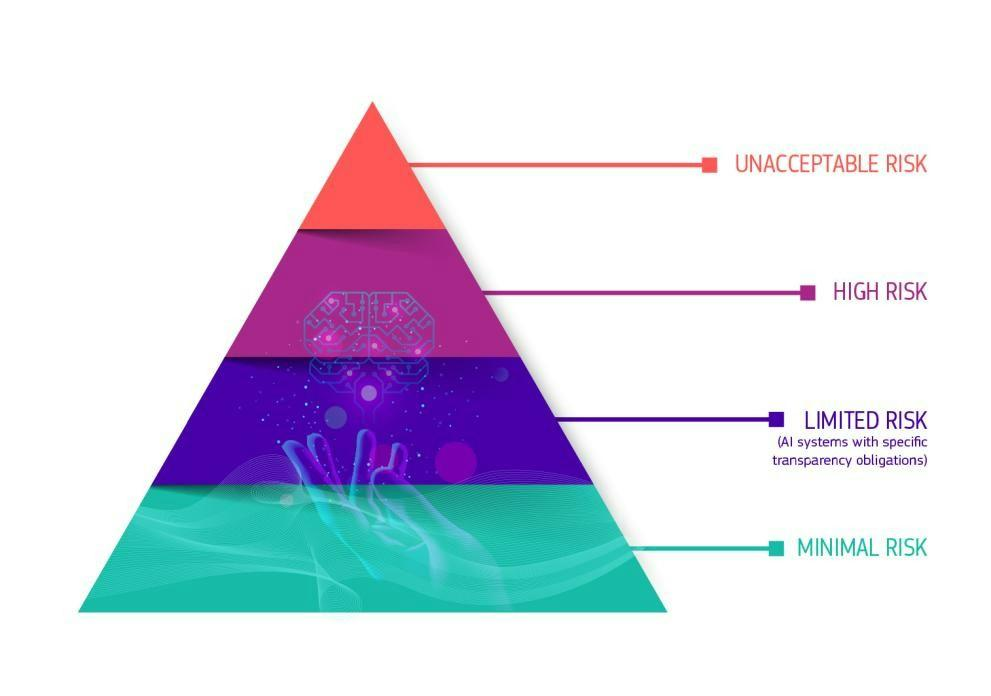
\includegraphics[scale=0.5]{./pictures/Pyramide.png}} 
    \end{center}
  \end{frame}


%% Darstellen der EU-Risikoklassen

\subsection{Erläuterung der Risikoklassen}
    \begin{frame} %{Erläuterung der Risikoklassen}
    \begin{center}

\begin{tabular}{|p{6.5cm}|@{}p{1cm}@{}|p{6.5cm}|}
    \hline
    \small
    \cellcolor{red!25}\textbf{Hochrisiko-Anwendungen} & \textbf{} & \cellcolor{red!50}\textbf{Unannehmbares Risiko} \\
    \hline
            \small
            \begin{itemize}
                \item Beeinflussen die Gesundheit, Sicherheit oder Lebenswege 
                \item Beispiele: KI in Stromkraftwerken, Kredit- und Jobentscheidungen (Art. 6)
                \item Unterscheidung: KI-Systeme für bereits geprüfte Produkte und andere Anwendungen (Art. 6 und Anhang III)
            \end{itemize}
            & & 

            \small
            \begin{itemize}
                \item Verboten: Systeme mit nicht akzeptablem Risiko 
                \item Beispiele: Verbot von staatlichen Social Scoring und schädlichen Manipulationssystemen (Art. 5) 
                \item Verbot für schädliche Systeme: Systeme, die darauf abzielen, Personen zu manipulieren oder deren Entscheidungsfindung zu beeinflussen (Art. 5)
            \end{itemize} \\
        \hline
    \end{tabular}

    \end{center}
\end{frame}

%%Darstellung Ungleichheit im Zugang zu technologischen Innovationen

\subsection{Ungleichheit im Zugang zu technologischen Innovationen}
\begin{frame} %{Ungleichheit im Zugang zu technologischen Innovationen}
    \centering
    
    
\includegraphics[width=0.2\textwidth]{./pictures/Fair.png}
    \hspace{1.0cm}
    
\includegraphics[width=0.2\textwidth]{./pictures/+.png}
    \hspace{1.0cm}
    
\includegraphics[width=0.2\textwidth]{./pictures/money.png}
    
    \vspace{0.2cm}
    
    \begin{minipage}[t]{0.2\textwidth}
      \centering
      \small moralische Gründe
    \end{minipage}
     \hspace{1.0cm}
    \begin{minipage}[t]{0.2\textwidth}
    \centering
    \small gesundheitliche Gründe
    \end{minipage}
    \hspace{1,0cm}
    \begin{minipage}[t]{0.2\textwidth}
    \centering
    \small finanzielle Gründe
    \end{minipage}
\end{frame}


%% Risiken in verschiedenn Ebenen
%% Risiken für Individuen
\subsection{Risiken für Individuen}
\begin{frame} %{Risiken für Individuen}
\centering
\renewcommand{\arraystretch}{1.5} % Erhöht den Zeilenabstand
\begin{tabular}{|p{12cm}|}
    \hline
    \rowcolor{blue!25}
    \textbf{Individuum} \\
    \hline
    \begin{itemize}
        \item Sicherheit der technischen Erweiterung (Hacking)
        \item Nutzer als Gefahr (Veränderung der Geräteeinstellung)
    \end{itemize} \\
    \hline
\end{tabular}
\end{frame}


%% Risiken für Organisationen
\subsection{Risiken für Organisationen}

\begin{frame} %{Risiken für Organisationen}
\centering
\renewcommand{\arraystretch}{1.5} % Erhöht den Zeilenabstand
\begin{tabular}{|p{12cm}|}
    \hline
    \rowcolor{blue!25}
    \textbf{Organisationen} \\
    \hline
    \begin{itemize}
        \item Abwägung des Risikos geprägt durch den // kapitalistischen Gedanken[24]
        \item Risiko durch Datenverkauf für "Neuro-Marketing" [24]
        \item Monopolbildung durch ungeregelten Vertrieb
    \end{itemize} \\
    \hline
\end{tabular}

\end{frame}

%% Riken für die Gesellschaft
\subsection{Risiken für die Gesellschaft}
\begin{frame} %{Risiken für die Gesellschaft}
\centering
\renewcommand{\arraystretch}{1.5} % Erhöht den Zeilenabstand
\begin{tabular}{|p{12cm}|}
    \hline
    \rowcolor{blue!25}
    \textbf{Gesellschaft} \\
    \hline
    \begin{itemize}
        \item Vorteilsbeschaffung bei Test oder im Sport[24]
        \item Militärischer Einsatz der Technik
        \item Verlust der Autonomie[24]
    \end{itemize} \\
    \hline
\end{tabular}

\end{frame}



%% Medizinische Vorteile in der Gegenwart

\subsection{Medizinische Vorteile in der Gegenwart}
\begin{frame} %{Medizinische Vorteile in der Gegenwart}
Verbesserung physischer und psychischer Leistungsfähigkeit\newline Heilen von:
	\begin{itemize}
		\item{Gehörlos}
		\item{Parkinson Erkrankten}
		\item{Tremor}
            \item{Chochlea-Implantatn}
            \item{Locked-in-Syndrom}
        \end{itemize}
\end{frame}


%% Medizinische Vorteile in der Zukungt

\subsection{Medizinische Vorteile in der Zukunft}
\begin{frame} %{Medizinische Vorteile in der Zukunft}
Heilen von Krankheiten (Transhumanismus)
	\begin{itemize}
		\item{psychisches Leiden}
		\item{Angststörung}
		\item{Depressionen}
            \item{Posttraumatische Belastungsstörungen}
            \item{Verbesserung der Leistungsfähigkeit}
        \end{itemize}
\end{frame}





% Zusammenfassung Vorteile und Nachteile

\subsection{Ist Transhumanismus Fortschritt oder Dystrophie?}
  \begin{frame} %{Ist Transhumanismus Fortschritt oder Dystrophie?}
    \begin{center}
    


\begin{tabular}{|p{6.5cm}|@{}p{1cm}@{}|p{6.5cm}|}
    \hline
    \cellcolor{green!40}\textbf{Vorteile} & \textbf{} & \cellcolor{red!50}\textbf{Nachteile} \\
            \small
            \begin{itemize}
                \item Erweterung der menschlichen Fähigkeiten
                \item Lösung von Gesundheitsproblemen
                \item Verbesserung der Lebensqualität
                \item Mögliche Evolution der Gesellschaft
            \end{itemize}
            & & 
            \begin{itemize}
                \item Unvorhersehbare Folgen
                \item Teilhabe, z.B. Arbeitsplatzverlust
                \item Ungleichheit
                \item Verlust der Menschlichkeit
                \item Datenschutz und Privatsphäre
            \end{itemize} \\
        \hline
    \end{tabular}

    \end{center}
\end{frame}

%\begin{frame}
\printbibliography % Druckt das Literaturverzeichnis in kleinerer Schriftgröße aus
%\end{frame}
\end{document}
